\chapter{Getting Started}
\label{chap:starting}
%HEVEA\cutname{starting.html}

\section{Hello Proofs}

The first step in using \why is to write a suitable input
file. When one wants to learn a programming language, one starts by
writing a basic program. Here is our first \why file, which is the file
\texttt{examples/logic/hello\_proof.why} of the distribution.
It contains a small set of goals.
\lstinputlisting[language=why3]{../examples/logic/hello_proof.why}

Any declaration must occur
inside a theory, which is in that example called HelloProof and
labeled with a comment inside double quotes. It contains three goals
named $G_1,G_2,G_3$. The first two are basic propositional goals,
whereas the third involves some integer arithmetic, and thus it
requires to import the theory of integer arithmetic from the \why
standard library, which is done by the \texttt{use} declaration above.

We don't give more details here about the syntax and refer to
Chapter~\ref{chap:syntax} for detailed explanations. In the following,
we show how this file is handled in the \why GUI
(Section~\ref{sec:gui}) then in batch mode using the \texttt{why3}
executable (Section~\ref{sec:batch}).

%EXECUTE rm -rf doc/hello_proof/
%EXECUTE cp examples/logic/hello_proof.why doc/

\section{Getting Started with the GUI}
\label{sec:gui}

The graphical interface allows to browse into a file or a set of
files, and check the validity of goals with external provers, in a
friendly way. This section presents the basic use of this GUI. Please
refer to Section~\ref{sec:ideref} for a more complete description.

%EXECUTE bin/why3 ide --batch "snap doc/gui-1.png" doc/hello_proof.why
\begin{figure}[tbp]
%HEVEA\centering
  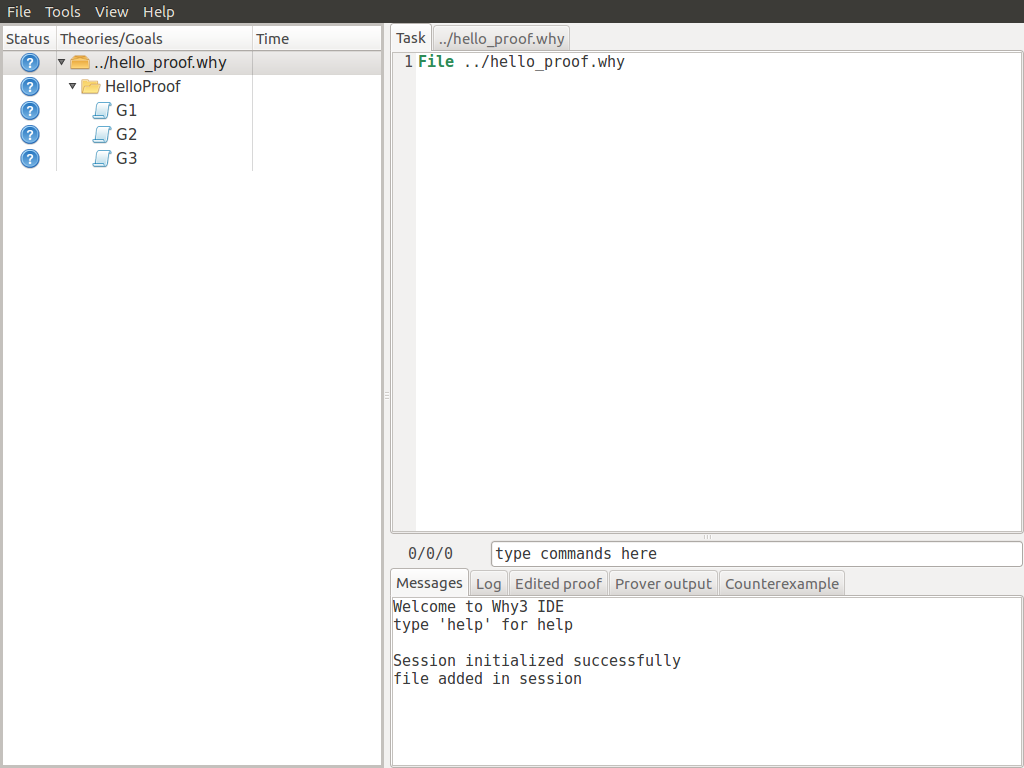
\includegraphics[width=\textwidth]{gui-1.png}
  \caption{The GUI when started the very first time.}
  \label{fig:gui1}
\end{figure}

The GUI is launched on the file above as follows
(here ``\texttt{>}'' is the prompt):
\begin{verbatim}
> why3 ide hello_proof.why
\end{verbatim}
When the GUI is started for the first time, you should get a window
that looks like the screenshot of Figure~\ref{fig:gui1}.
The left part is a tree view that
allows to browse inside the theories.
% Initially, the item of this tree
% are closed. We can expand this view using the menu \textsf{View/Expand
%   all} or its shortcut \textsf{Ctrl-E}. This will result is something
% like the screenshot of Figure~\ref{fig:gui2}.
In this tree view, we have a structured view of the file: this file
contains one theory, itself containing three goals.
%EXECUTE bin/why3 ide --batch "type next;snap -crop 1024x384+0+0 doc/gui-2.png" doc/hello_proof.why
\begin{figure}[tbp]
%HEVEA\centering
 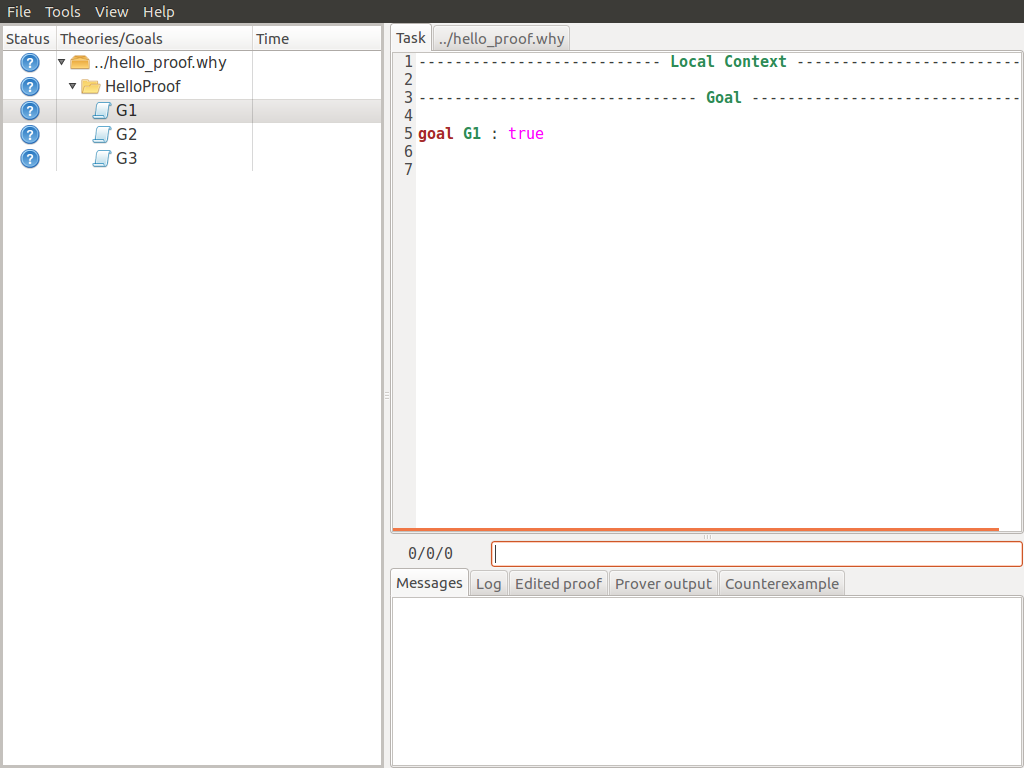
\includegraphics[width=\textwidth]{gui-2.png}
  \caption{The GUI with goal G1 selected.}
  \label{fig:gui2}
\end{figure}
In Figure~\ref{fig:gui2}, we clicked on the row corresponding to
goal $G_1$. The \emph{task} associated with this goal is then
displayed on the top right, and the corresponding part of the input
file is shown on the bottom right part.


\subsection{Calling provers on goals}

You are now ready to call provers on the goals
%BEGIN LATEX
\footnote{If not done yet, you
  must perform prover autodetection using \texttt{why3 config
    -{}-detect-provers}}.
%END LATEX
%HEVEA {} (If not done yet, you must perform prover autodetection using \texttt{why3 config -{}-detect-provers}.)
A prover is selected using the context menu (right-click), in the
\texttt{Provers} sub-menu.
This prover is then called on the goal selected
in the tree view. You can select several goals at a time, either
by using multi-selection (typically by clicking while pressing the
\textsf{Shift} or \textsf{Ctrl} key) or by selecting the parent theory
or the parent file.

Let us now select the theory ``HelloProof'' and
run the Alt-Ergo prover. After a short time, you should
get the display of Figure~\ref{fig:gui3}.
%EXECUTE bin/why3 ide --batch "type alt-ergo;view source;wait 3;snap -crop 1024x384+0+0 doc/gui-3.png" doc/hello_proof.why
\begin{figure}[tbp]
%HEVEA\centering
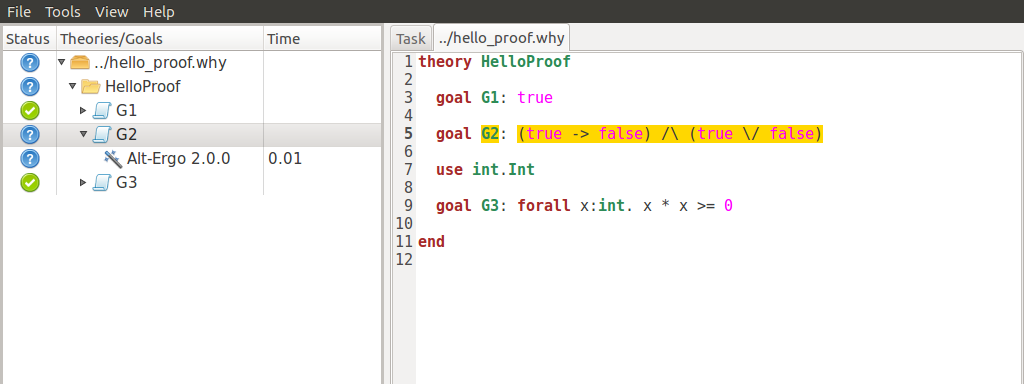
\includegraphics[width=\textwidth]{gui-3.png}
  \caption{The GUI after running the Alt-Ergo prover on each goal.}
  \label{fig:gui3}
\end{figure}
Goals $G_1$ and $G_3$ are now marked with a green ``checked'' icon in the
status column. This means that these goals have been proved by Alt-Ergo.
On the contrary, goal $G_2$ is not proved; it remains
marked with a question mark.
You could attempt to prove $G_2$ using another prover, though it is
obvious here it will not succeed.

\subsection{Applying transformations}

Instead of calling a prover on a goal, you can apply a transformation
to it.  Since $G_2$ is a conjunction, a possibility is to split it
into subgoals. You can do that by selecting \textsf{Split} in the
\texttt{Strategies} sub-menu of the context menu. Now you have two
subgoals, and you can try again a prover on them, for example
Alt-Ergo. We already have a lot of goals and proof attempts, so it is
a good idea to close the sub-trees which are already proved: this can
be done by the menu \textsf{View/Collapse proved goals}, or even
better by its shortcut ``Ctrl-C''.  You should see now what is
displayed on Figure~\ref{fig:gui4}.

%EXECUTE bin/why3 ide --batch "type alt-ergo;wait 3;type next;type split_goal_wp;wait 1;snap -crop 1024x384+0+0 doc/gui-4.png;save;wait 1" doc/hello_proof.why
\begin{figure}[tbp]
%HEVEA\centering
 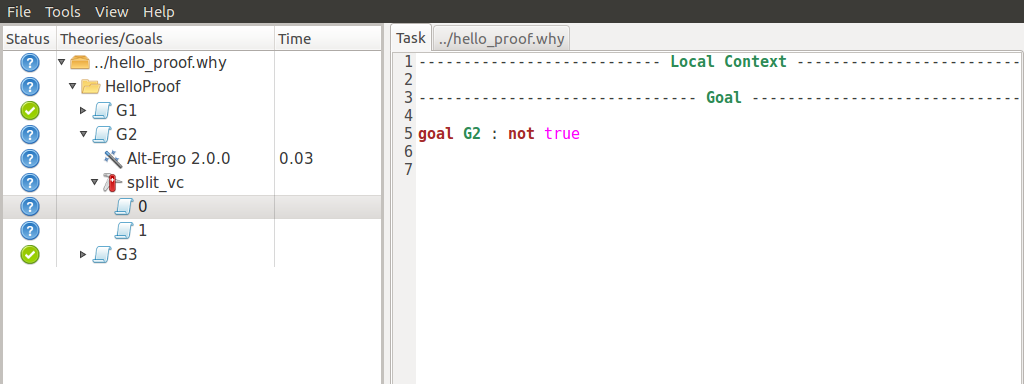
\includegraphics[width=\textwidth]{gui-4.png}
  \caption{The GUI after splitting goal $G_2$.}
  \label{fig:gui4}
\end{figure}

The first part of goal $G_2$ is still unproved. As a last resort, we
can try to call the Coq proof assistant, by selecting it in the
\texttt{Provers} list.
A new sub-row appear for Coq, and the Coq proof editor is launched.
(It is \texttt{coqide} by default; see
Section~\ref{sec:ideref} for details on how to configure this). You get
now a regular Coq file to fill in, as shown on Figure~\ref{fig:coqide}.
Please be mindful of the comments of this file. They indicate where \why
expects you to fill the blanks. Note that the comments themselves should
not be removed, as they are needed to properly regenerate the file when the
goal is changed. See Section~\ref{sec:coq} for more details.

\begin{figure}[tbp]
%HEVEA\centering
  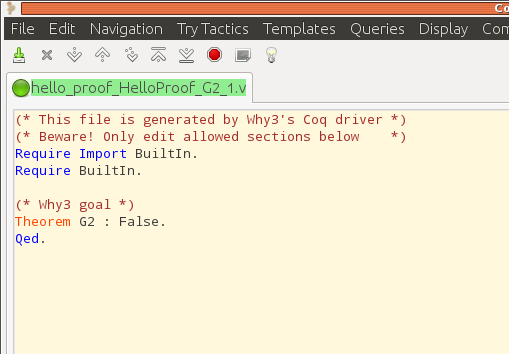
\includegraphics[width=\textwidth]{coqide-0-81.png}
  \caption{CoqIDE on subgoal 1 of $G_2$}
  \label{fig:coqide}
\end{figure}

Of course, in that particular case, the goal cannot be proved since it
is not valid. The only thing to do is to fix the input file, as
explained below.

\subsection{Modifying the input}

You can edit the source file, using the corresponding tab in the
top-right window of the GUI.
Let us assume we
change the goal $G_2$ by replacing the first occurrence of \texttt{true} by
\texttt{false}, \eg
\begin{whycode}
  goal G2 : (false -> false) /\ (true \/ false)
\end{whycode}
We can refresh the goals using menu \textsf{File/Save all and Refresh
  session}, or the shortcut ``Ctrl-R''. We get the tree view shown on
Figure~\ref{fig:gui5}.

%EXECUTE bin/why3 ide --batch "type next;type coq;wait 1;save;wait 1" doc/hello_proof.why
%EXECUTE sed -i -e 's/true -> false/false -> false/' doc/hello_proof.why
%EXECUTE bin/why3 ide --batch "type next;type expand;snap -crop 1024x384+0+0 doc/gui-5.png" doc/hello_proof.why
\begin{figure}[tbp]
%HEVEA\centering
  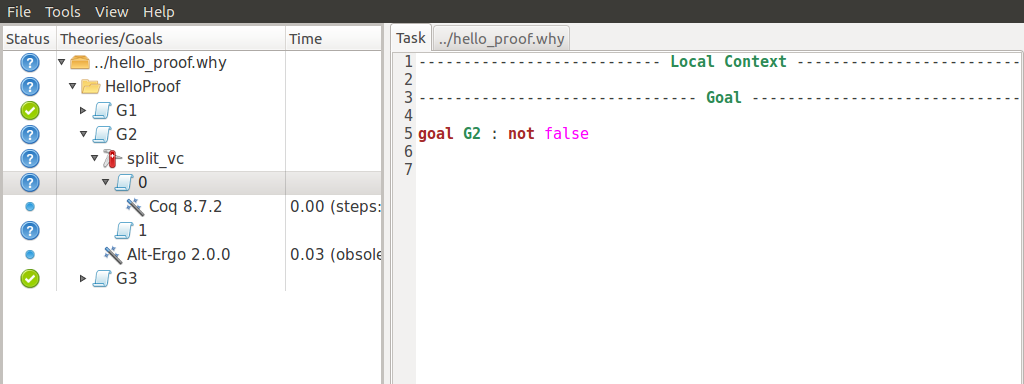
\includegraphics[width=\textwidth]{gui-5.png}
  \caption{File reloaded after modifying goal $G_2$}
  \label{fig:gui5}
\end{figure}

The important feature to notice first is that all the previous proof
attempts and transformations were saved in a database --- an XML file
created when the \why file was opened in the GUI for the first
time. Then, for all the goals that remain unchanged, the previous
proofs are shown again. For the parts that changed, the previous
proofs attempts are shown but marked with ``(obsolete)''\index{obsolete!proof attempt}
so that you
know the results are not accurate. You can now retry to prove all what
remains unproved using any of the provers.

\subsection{Replaying obsolete proofs}

Instead of pushing a prover's button to rerun its proofs, you can
\emph{replay} the existing but obsolete
proof attempts, using menu
\textsf{Tools/Replay obsolete}. By default, \textsf{Replay} only replays
proofs that were successful before.
%% FIXME? ça existe toujours dans le nouvel IDE ?
% If you want to replay all of them,
% you must select the context \textsf{all goals} at the top of the left
% tool bar.

Notice that replaying can be done in batch mode, using the
\texttt{replay} command (see Section~\ref{sec:why3replayer}) For
example, running the replayer on the \texttt{hello\_proof} example is
as follows (assuming $G_2$ still is
\lstinline|(true -> false) /\ (true \/ false)|).
\begin{verbatim}
> why3 replay hello_proof
 2/3 (replay OK)
   +--file ../hello_proof.why: 2/3
      +--theory HelloProof: 2/3
         +--goal G2 not proved
\end{verbatim}
The last line tells us that no differences were detected between the
current run and the run stored in the XML file. The tree above
reminds us that $G_2$ is not proved.

\subsection{Cleaning}

You may want to clean some the proof attempts, \eg removing the
unsuccessful ones when a project is finally fully proved.
A proof or a transformation can be removed by selecting it and
using menu \textsf{Tools/Remove} or key \texttt{Suppr}.
It performs an automatic removal of all proofs
attempts that are unsuccessful, while there exists a successful proof
attempt for the same goal.
Beware that there is no way to undo such a removal.

\section{Getting Started with the \why Command}
\label{sec:batch}

The \texttt{prove} command makes it possible to check the validity of goals with external
provers, in batch mode. This section presents the basic use of this
tool. Refer to Section~\ref{sec:why3ref} for a more complete
description of this tool and all its command-line options.

The very first time you want to use \why, you should proceed with
autodetection of external provers.
%% We have already seen how to do it in the \why GUI.
On the command line, this is done as follows:
\begin{verbatim}
> why3 config --detect
\end{verbatim}
This prints some information messages on what detections are attempted. To know which
provers have been successfully detected, you can do as follows.
\begin{verbatim}
> why3 --list-provers
Known provers:
  Alt-Ergo 1.30
  CVC4 1.5
  Coq 8.6
\end{verbatim}
\index{list-provers@\verb+--list-provers+}
The first word of each line
is a unique identifier for the associated prover. We thus have now the
three provers Alt-Ergo~\cite{ergo}, CVC4~\cite{cvc4}, and
Coq~\cite{CoqArt}.

Let us assume that we want to run Alt-Ergo on the HelloProof
example. The command to type and its output are as follows, where the
\verb|-P| option is followed by the unique prover identifier (as shown
by \verb|--list-provers| option).
\begin{verbatim}
> why3 prove -P Alt-Ergo hello_proof.why
hello_proof.why HelloProof G1: Valid (0.00s, 1 steps)
hello_proof.why HelloProof G2: Unknown (other) (0.01s)
hello_proof.why HelloProof G3: Valid (0.00s, 1 steps)
\end{verbatim}
Unlike the \why GUI, the command-line tool does not save the proof attempts
or applied transformations in a database.

We can also specify which goal or goals to prove. This is done by giving
first a theory identifier, then goal identifier(s). Here is the way to
call Alt-Ergo on goals $G_2$ and $G_3$.
\begin{verbatim}
> why3 prove -P Alt-Ergo hello_proof.why -T HelloProof -G G2 -G G3
hello_proof.why HelloProof G2 : Unknown: Unknown (0.01s)
hello_proof.why HelloProof G3 : Valid (0.01s)
\end{verbatim}

Finally, a transformation to apply to goals before proving them can be
specified. To know the unique identifier associated to
a transformation, do as follows.
\begin{verbatim}
> why3 --list-transforms
Known non-splitting transformations:
  [...]

Known splitting transformations:
  [...]
  split_goal_right
\end{verbatim}
Here is how you can split the goal $G_2$ before calling
Simplify on the resulting subgoals.
\begin{verbatim}
> why3 prove -P Alt-Ergo hello_proof.why -a split_goal_right -T HelloProof -G G2
hello_proof.why HelloProof G2: Unknown (other) (0.01s)
hello_proof.why HelloProof G2: Valid (0.00s, 1 steps)
\end{verbatim}
Section~\ref{sec:transformations} gives the description of the various
transformations available.

%EXECUTE rm -r doc/hello_proof.why doc/hello_proof/

%%% Local Variables:
%%% mode: latex
%%% TeX-PDF-mode: t
%%% TeX-master: "manual"
%%% End:
